\documentclass{article}
\usepackage[utf8]{inputenc}
\usepackage{vmargin}


\usepackage{amsmath} 
\usepackage{graphicx}
\usepackage{graphics}
\usepackage{float}
\usepackage{blindtext}
\usepackage{listings}
\usepackage{xcolor}
\usepackage[spanish]{babel}
\usepackage{subfig}

\graphicspath{ {images/} }
\title{Operador Logarítmico}
\date{}
\setpapersize{A4}
\setmargins{2.5cm}       % margen izquierdo
{1.5cm}                        % margen superior
{16.5cm}                      % anchura del texto
{23.42cm}                    % altura del texto
{10pt}                           % altura de los encabezados
{1cm}                           % espacio entre el texto y los encabezados
{0pt}                             % altura del pie de página
{2cm}                           % espacio entre el texto y el pie de página

\begin{document}

%-------COLORES PARA CODIGO ------------------------
\lstdefinestyle{customc}{
  belowcaptionskip=1\baselineskip,
  breaklines=true,
  frame=L,
  xleftmargin=\parindent,
  language=JavaScript,
   basicstyle=\footnotesize\ttfamily,
  showstringspaces=false,
  basicstyle=\footnotesize\ttfamily,
  keywordstyle=\bfseries\color{green!40!black},
  commentstyle=\itshape\color{purple!40!black},
  identifierstyle=\color{blue},
  stringstyle=\color{orange},
  frame=single,	  
  numbers=left,
   numberstyle=\footnotesize,
}

\lstdefinestyle{customasm}{
  belowcaptionskip=1\baselineskip,
  frame=L,
  xleftmargin=\parindent,
  language=JavaScript,
  basicstyle=\footnotesize\ttfamily,
  commentstyle=\itshape\color{purple!40!black},
}

\lstset{escapechar=@,style=customc}

%---------------------------------------------

\thispagestyle{empty}

\vfill
 \begin{center}
    \begin{figure}[h]
    \centering
    \includegraphics[width=12cm]{unsa}\\
    
    \end{figure}
 	 
     \vspace*{1.5cm}
    {\large\bfseries FACULTAD DE PRODUCCIÓN Y SERVICIOS} \\
    {\large\bfseries ESCUELA PROFESIONAL DE CIENCIA DE LA COMPUTACIÓN}  \\    
    \vspace*{1.5cm}
    
 	\rule[0.5ex]{\linewidth}{2pt}\vspace*{-\baselineskip}\vspace*		{3.2pt}
	\rule[0.5ex]{\linewidth}{1pt}\\[\baselineskip]
 	{\huge Física Computacional} \\[4mm]
    \rule[0.5ex]{\linewidth}{1pt}\vspace*{-							\baselineskip}\vspace{3.2pt}
	\rule[0.5ex]{\linewidth}{2pt}\\
 	\vspace*{1cm}

    \begin{large} \bfseries
    Tarea Movimiento Oscilatorio \\
    
    \vspace{5mm}
    Eduardo Antonio Sánchez Hincho \\

    \vspace{5mm}
    Docente:\\
    Edwin Agapito Llamoca Requena
    \end{large}
    \vspace*{0.4in}
    
    \noindent \\
    
    \vfill
    \large\bfseries{ AREQUIPA\\2020}
\end{center}
\newpage
\section{Problemas}
\subsection{1}
Se implementó el siguiente código para todas las gráficas
\begin{lstlisting}[language=Python,caption=Desafío 1.1]
h = 0.001
k = 0.1
m = 0.2

px = 2
pos = []

velo = 0
velocidad = []

aceleracion = []

tiempo = 50
pt = np.arange(0, tiempo, h)

U = []
K = []
E = []

for i in pt:

    pos.append(px)
    velocidad.append(velo)
    aceleracion.append((-k/m)*px)

    velo = velo + aceleracion[-1]*h
    px = px + velo*h
    
    U.append((1/2)*k*pos[-1]**2)
    K.append((1/2)*m*velocidad[-1]**2)
    E.append(U[-1]+K[-1])
\end{lstlisting}

\subsubsection{Gráfico a}
\begin{figure}[H]
    \centering
    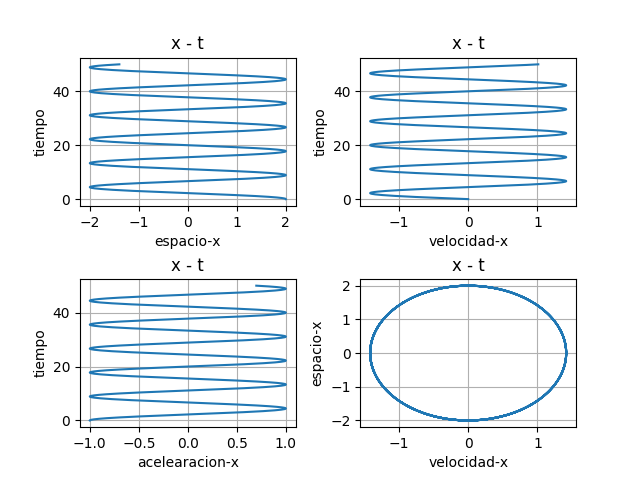
\includegraphics[width=0.6\textwidth]{Figure_1.png}
    \caption{Resultado}
\end{figure}

\subsubsection{Gráfico b}
\begin{figure}[H]
    \centering
    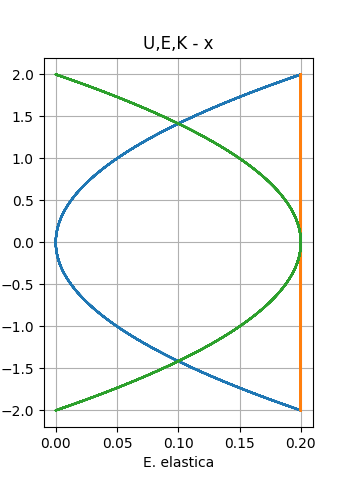
\includegraphics[width=0.4\textwidth]{Figure_2.png}
    \caption{Resultado}
\end{figure}

\subsubsection{Gráfico c}
\begin{figure}[H]
    \centering
    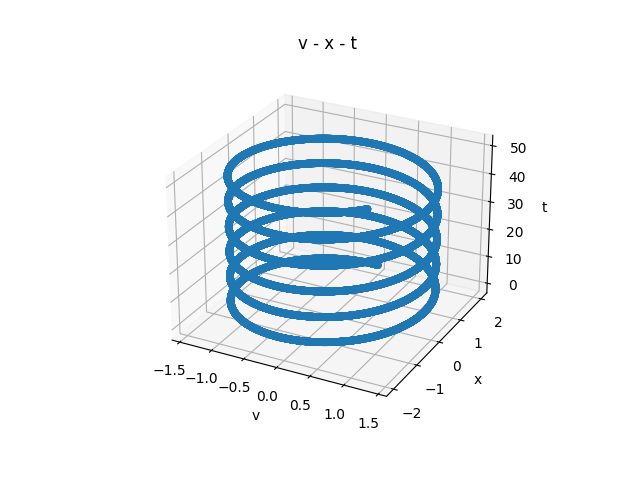
\includegraphics[width=0.7\textwidth]{Figure_3.png}
    \caption{Resultado}
\end{figure}
\newpage
\subsection{2}
\begin{lstlisting}[language=Python,caption=Desafío 1.1]
k = 0.1
m = 0.2
f0 = 0
c = 0.05
w = 0

h = 0.01
t = 40

ax = 0
x = 0
vx = -2

pos = []
velocidad = []
aceleracion = []

U = []
K = []
E = []

pt = np.arange(0,t,h)
ax = -k*x/m-c*vx/m+f0*np.cos(w*t)/m
vx = vx+ax*h/2


for t in pt:
    ax = -k*x/m-c*vx/m+f0*np.cos(w*t)/m
    vx = vx+ax*h
    x = x+vx*h

    pos.append(x)
    velocidad.append(vx)
    aceleracion.append(ax)

    U.append(k*(x*x)/2)
    K.append(m*(vx*vx)/2)
    E.append(u[-1]+K[-1])

\end{lstlisting}

\subsubsection{Gráfico a}
\begin{figure}[H]
    \centering
    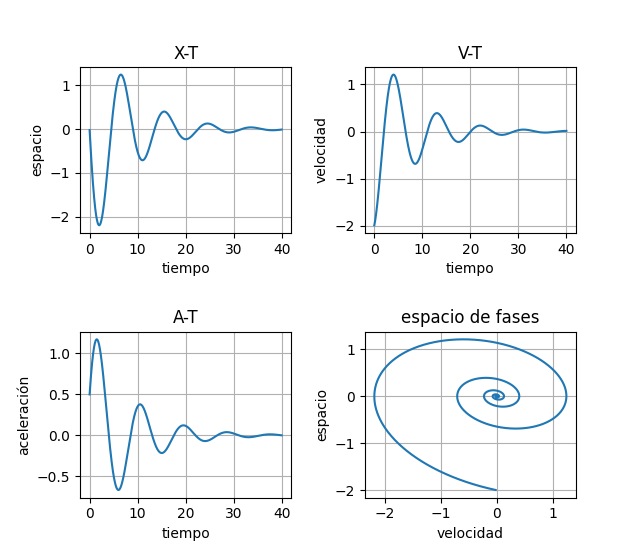
\includegraphics[width=0.7\textwidth]{Figure_2_1.png}
    \caption{Resultado}
\end{figure}

\subsubsection{Gráfico b}
\begin{figure}[H]
    \centering
    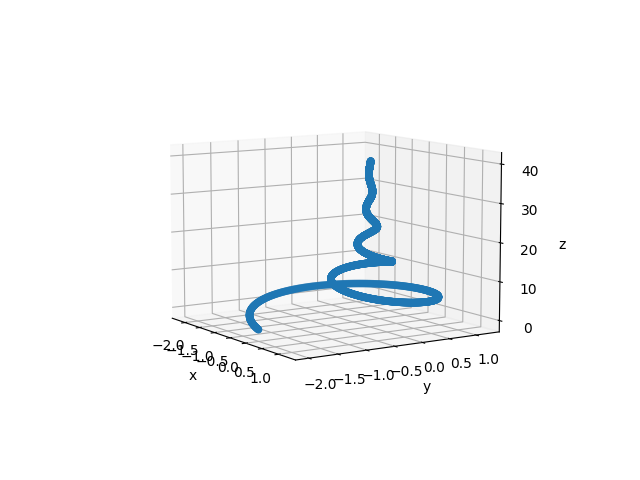
\includegraphics[width=0.7\textwidth]{Figure_2_2.png}
    \caption{Resultado}
\end{figure}

\subsection{3}
\begin{lstlisting}[language=Python,caption=Desafío 1.1]
k = 0.1
m = 0.2
f0 = 0.01
c = 0.05
w = 0.3

h = 0.01
t = 40

ax = 0
x = -1
vx = 1

pos = []
velocidad = []
aceleracion = []

U = []
K = []
E = []

pt = np.arange(0,t,h)
ax = -k*x/m-c*vx/m+f0*np.cos(w*t)/m
vx = vx+ax*h/2


for t in pt:
    ax = -k*x/m-c*vx/m+f0*np.cos(w*t)/m
    vx = vx+ax*h
    x = x+vx*h

    pos.append(x)
    velocidad.append(vx)
    aceleracion.append(ax)

    U.append(k*(x*x)/2)
    K.append(m*(vx*vx)/2)
    E.append(u[-1]+K[-1])
\end{lstlisting}
\subsubsection{Gráfico a}
\begin{figure}[H]
    \centering
    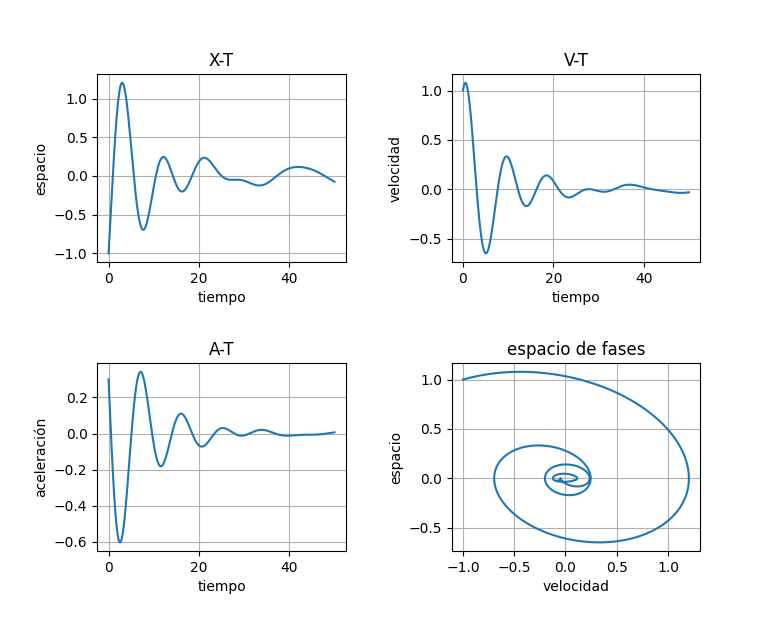
\includegraphics[width=0.7\textwidth]{Figure_3_1.png}
    \caption{Resultado}
\end{figure}

\subsubsection{Gráfico b}
\begin{figure}[H]
    \centering
    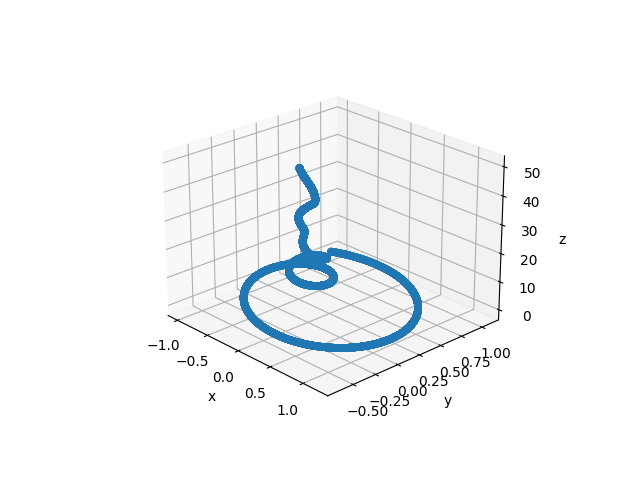
\includegraphics[width=0.7\textwidth]{Figure_3_2.png}
    \caption{Resultado}
\end{figure}

\section{Desafío}
\begin{lstlisting}[language=Python,caption=Desafío 1.1]
k = 0.1
m = 0.2
c = 0.05
w = 0.3
f0 = 0.01
f1 = 0

h = 0.01
t = 100

ax = 0
ax1 = 0

x = -1
x1 = -1

vx = 1
vx1 = 1

pos = []
pos1 = []

velocidad = []
velocidad1 = []

aceleracion = []
aceleracion1 = []

ax = -k*x/m-c*vx/m+f0*np.cos(w*t)/m
vx = vx+ax*h/2

ax1 = -k*x1/m-c*vx1/m+f1*np.cos(w*t)/m
vx1 = vx1+ax1*h/2

pt=np.arange(0,t,h)

for t in pt:
    ax = -k*x/m-c*vx/m+f0*np.cos(w*t)/m
    vx = vx+ax*h
    x = x+vx*h
    
    ax1 = -k*x1/m-c*vx1/m+f1*np.cos(w*t)/m
    vx1 = vx1+ax1*h
    x1 = x1+vx1*h
    
   
    pos.append(x)
    velocidad.append(vx)
    aceleracion.append(ax)

    pos1.append(x1)
    velocidad1.append(vx1)
    aceleracion1.append(ax1)
\end{lstlisting}
\subsection{1}
\begin{figure}[H]
    \centering
    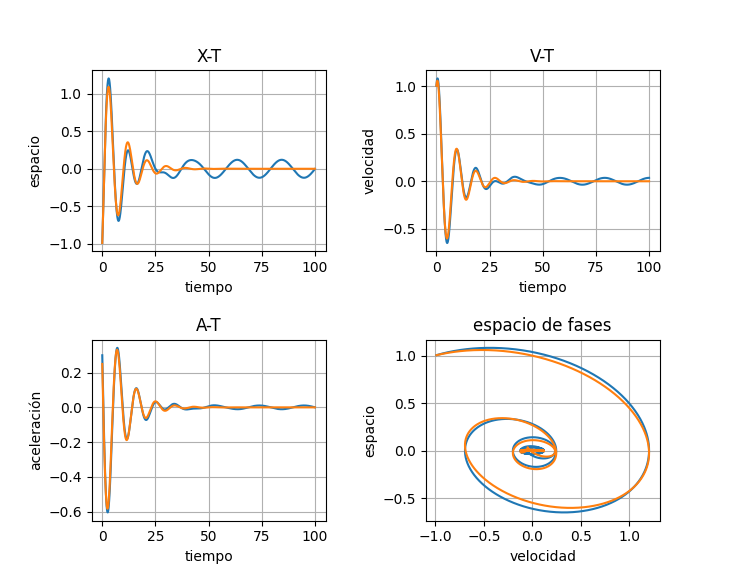
\includegraphics[width=0.7\textwidth]{desa1.png}
    \caption{Resultado}
\end{figure}

\subsection{2}
\begin{figure}[H]
    \centering
    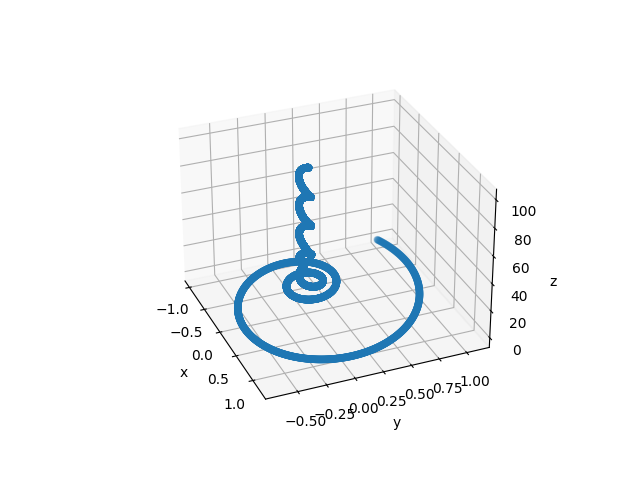
\includegraphics[width=0.7\textwidth]{desa2.png}
    \caption{Resultado}
\end{figure}

\subsection{3}
\begin{figure}[H]
    \centering
    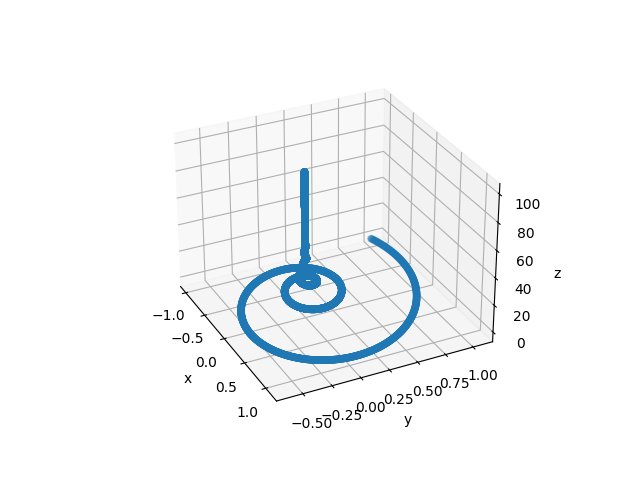
\includegraphics[width=0.7\textwidth]{desa3.png}
    \caption{Resultado}
\end{figure}

\end{document}


